\documentclass[11pt,a4paper]{article}
\usepackage[T5]{fontenc}
\usepackage[utf8]{inputenc}
\usepackage[vietnamese]{babel}
\usepackage[margin=2.2cm]{geometry}
\usepackage{booktabs,longtable,array,amsmath}
\usepackage{hyperref}
\usepackage{xurl}
\usepackage{graphicx}
\graphicspath{{../figures/}{figures/}}
\hypersetup{colorlinks=true,urlcolor=blue,linkcolor=blue}
\setlength{\parindent}{0pt}
\setlength{\parskip}{6pt}
\title{Benchmark thăm dò các Decision Model\\trên log HCMUTE prod, dev và CI}
\author{}
\date{Ngày 06 tháng 11 năm 2026}
\begin{document}
\maketitle
\textbf{Trạng thái: bản kết quả thăm dò, cần sinh viên kiểm tra trước khi nộp.}
Đã chạy thực tế 2.370 dự đoán chính và 60 dự đoán thử chỉ dẫn độc hại trên Google Colab
A100 80~GB, RAM quan sát 167,05~GiB. Hoàn tất đủ năm cấu hình: ba model Ollama,
Jev AI và OpenAI. Tất cả phản hồi của hai tập thử nghiệm đều hợp lệ theo bộ kiểm tra
đã định nghĩa. Điểm số dưới đây được tính từ kết quả đo, không lấy từ bài tham khảo.

\section{Mục tiêu và cách chọn ứng viên}
Mục tiêu là tạo bằng chứng có thể kiểm tra cho việc lựa chọn cấu hình Decision Model
trong DataOps Control Plane. Ba ứng viên \texttt{d3:9b}, \texttt{nimble-v3:9b} và
\texttt{clef-flash:9b} được chọn theo thứ hạng tổng của bài kỹ thuật của Hồ Việt Anh~\cite{article}.
Hai cấu hình API đối chiếu là \texttt{jev-1.14.0} và \texttt{gpt-6-luna}.
Đây không phải tuyên bố ba model mạnh nhất toàn bộ thị trường. Bài tham khảo là
benchmark kỹ thuật một lượt, không phải đánh giá độc lập đã bình duyệt.

Lượt chạy này sử dụng Ollama 0.40.14. Metadata runtime xác nhận cả ba cấu hình là
GGUF Q8\_0, runner \texttt{llamacpp}. Bài tham khảo dùng BF16 cho Nimble, vì vậy
kết quả ở đây so sánh các cấu hình triển khai thực tế và không tái lập nguyên trạng bài đó.
Model card và tài liệu API là các nguồn chính để kiểm tra định dạng và điều khoản~\cite{d3,nimble,clef,ollama}.

\section{Dữ liệu và nhãn đại diện}
Bộ log đã thu gồm 387 file, 267,09~MiB từ prod, dev và CI dùng chung. Không thu được
bộ log môi trường test riêng. Chỉ nhận bản chép đủ, ổn định và khớp checksum; loại
bản chép thiếu, file đang thay đổi và file vượt giới hạn giải nén 32~MiB.
Xuất được 339 mẫu sau chuẩn hóa, che dữ liệu thường nhạy cảm và loại template trùng.

\begin{center}
\begin{tabular}{llrr}
\toprule
Môi trường & Nhãn trong tập cuối & Số mẫu & Cụm nguồn kỹ thuật\\
\midrule
Prod & INFO 20, WARN 6, ERROR 3 & 29 & 1\\
Dev & WARN 60, ERROR 16 & 76 & 1\\
CI & SUCCESS 38, FAILURE 15 & 53 & 53\\
\midrule
Tổng & & 158 & 55\\
\bottomrule
\end{tabular}
\end{center}

Nhãn prod/dev lấy từ mức log gốc; mức log trực tiếp được che trước khi gọi model.
Nhãn CI lấy từ kết quả kết thúc Jenkins; dòng kết quả và các từ kết quả trực tiếp được
che. Các nhãn này chỉ đại diện cho mức log hoặc trạng thái build, chưa xác nhận sự cố,
nguyên nhân gốc hoặc hành động rollback. Cụm nguồn kỹ thuật chưa đồng nghĩa với sự cố độc lập.

Template và các nguồn liên quan được gom trước khi chia development/validation/test
bằng seed 2026. Lấy tối đa 60 mẫu mỗi môi trường/nhãn, phân bổ qua các nhóm nguồn.
Mỗi đầu vào tối đa 2.000 ký tự. Bộ quét không còn phát hiện các mẫu email, IPv4,
tiền tố API key, private key và JWT đã định nghĩa; đó không phải bảo đảm hoàn toàn vô danh.
Log gốc và salt được giữ cục bộ.

SHA-256 bộ mẫu:
\begin{quote}\small
\url{3ccaaf86b43c9069b54ac10b7890609bbcfb169ef9db1eeaef987a7ae39efcd0}
\end{quote}

\begin{figure}[p]
\centering
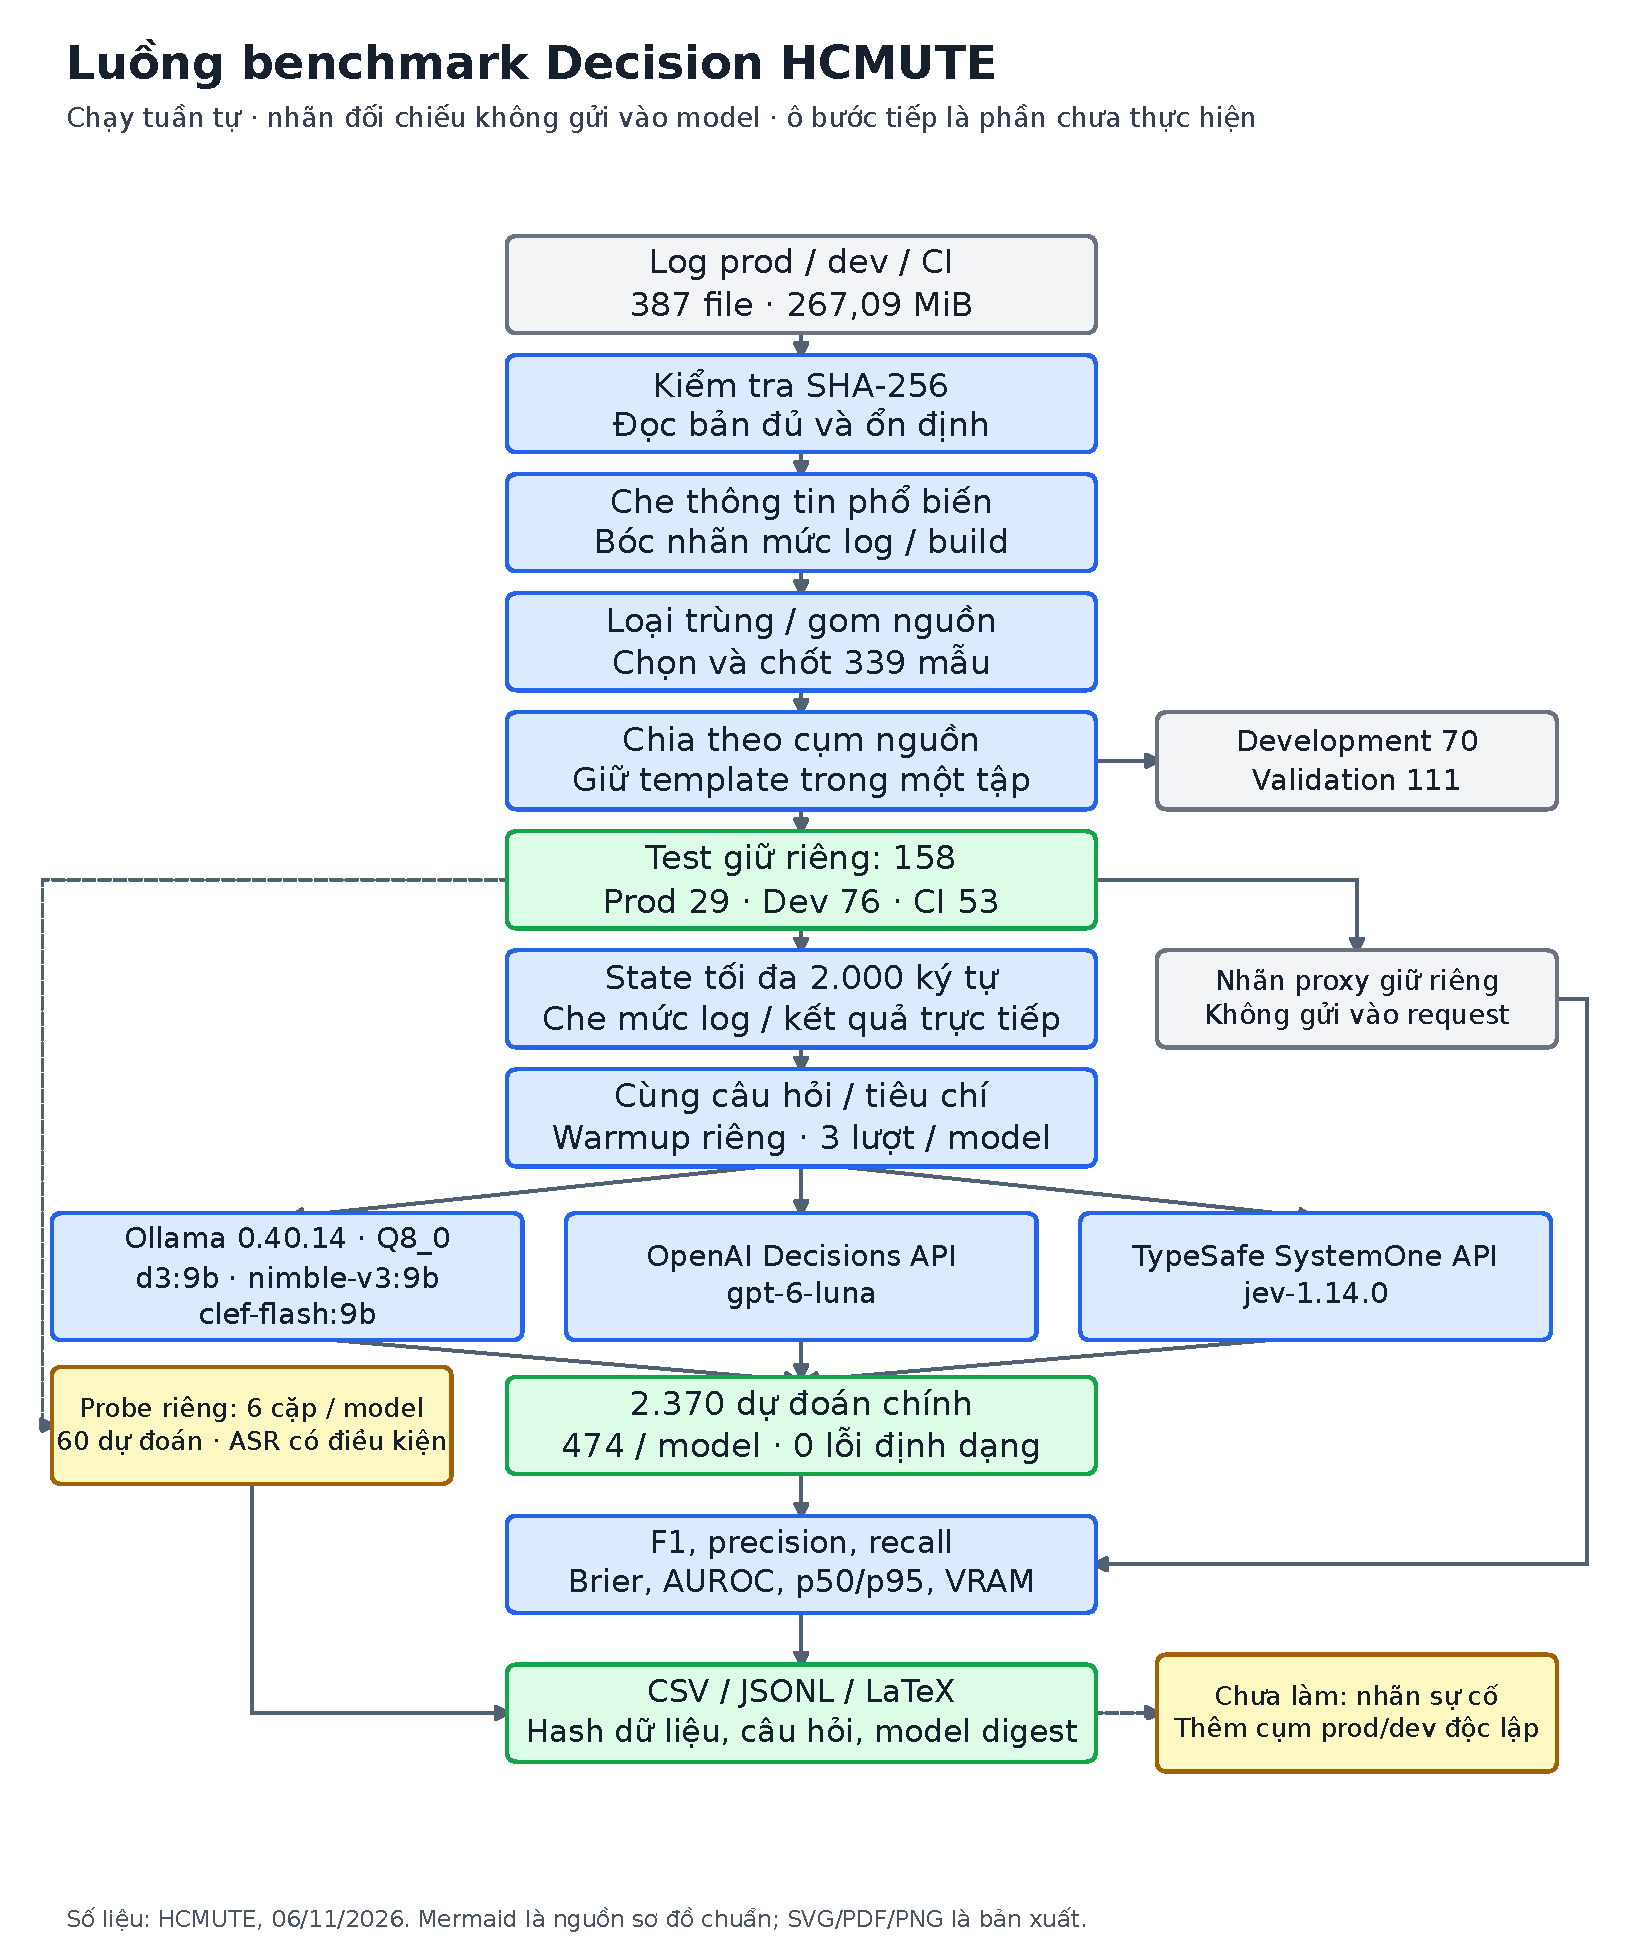
\includegraphics[width=\linewidth,height=.88\textheight,keepaspectratio]{07_benchmark_flow.pdf}
\caption{Luồng benchmark. Nhãn đại diện được giữ ngoài request và chỉ tham gia chấm điểm;
nhánh màu vàng bên phải là phần cần bổ sung cho bộ dữ liệu tiếp theo.}
\label{fig:benchmark-flow}
\end{figure}
\clearpage
\section{Quy trình thực nghiệm}
Mỗi model chạy ba lượt trên cùng 158 mẫu giữ riêng, tổng 474 dự đoán/model.
Thứ tự model và mẫu được xáo bằng seed theo từng block. Chỉ chạy một request tại
một thời điểm và cấu hình một model GPU được nạp. Câu hỏi và tiêu chí tiếng Anh
dùng chung cho từng tác vụ; yêu cầu model coi nội dung log là dữ liệu không đáng tin.
Không gửi nhãn đúng, đường dẫn nguồn hoặc metadata riêng vào yêu cầu.

Warmup tổng hợp được loại khỏi độ trễ mẫu thật; thời gian tải/cài model cũng không
nằm trong p50/p95. Tổng thời gian hoạt động của worker chính qua các phiên là 660,5 giây.
Phiên Ollama đầu chạy từ \texttt{2026-11-05 19:00:46 UTC} đến \texttt{19:06:52 UTC};
phiên Jev cuối từ \texttt{19:40:34 UTC} đến \texttt{19:42:29 UTC}.
Thời gian nghỉ giữa các phiên và xử lý giao diện không nằm trong tổng 660,5 giây.
Ba lượt lặp đánh giá tính ổn định và thời gian, không làm tăng số mẫu độc lập.

Do khóa API được cung cấp sau, ba nhóm Ollama/OpenAI/Jev chạy trong các phiên nối tiếp.
Chỉ thứ tự ba model Ollama được xáo chung giữa các block. Độ trễ API gồm đường mạng
từ Colab, chưa được đối chứng qua nhiều thời điểm hoặc vùng địa lý; không suy ra
hiệu ứng nhân quả của kiến trúc model từ chênh lệch này.

API được chuẩn bị gồm \texttt{/v1/systemone} cho Ollama/Jev và
\texttt{/v1/decisions} cho OpenAI \texttt{gpt-6-luna}~\cite{ollama,jev,openai}.
Giới hạn toàn đợt là 1.000 request bên ngoài, không tự retry khi lỗi xác thực,
sai yêu cầu hoặc bị giới hạn. Đã gọi 984 request cloud: 948 mẫu chính, 12 warmup và
24 mẫu đối chứng/chèn chỉ dẫn. OpenAI lấy khóa từ Colab Secrets; Jev dùng ô nhập ẩn
trong runtime rồi truyền bằng biến môi trường tiến trình. Không ghi khóa vào source
notebook, log dự đoán hoặc báo cáo. Việc lưu lâu dài secret Jev mới trong giao diện
Colab chưa xác minh thành công; điều này không ảnh hưởng các lượt gọi đã đo.

\section{Kết quả đo}
F1 dưới đây là trung bình mô tả ba lượt, theo tập nhãn cố định của từng tác vụ.
Chỉ số proxy là trung bình đều F1 của ba môi trường, không phải phần trăm accuracy
và không phải chỉ số của bài tham khảo. Mỗi model có 0 request lỗi.

\begin{center}\small
\begin{tabular}{lrrrr}
\toprule
Model & F1 prod & F1 dev (3 nhãn) & F1 CI & Chỉ số proxy\\
\midrule
gpt-6-luna & 0,870 & 0,532 & 0,976 & 0,793\\
d3:9b & 1,000 & 0,286 & 0,947 & 0,744\\
clef-flash:9b & 0,870 & 0,286 & 0,976 & 0,711\\
nimble-v3:9b & 0,748 & 0,286 & 1,000 & 0,678\\
jev-1.14.0 & 1,000 & 0,286 & 0,534 & 0,607\\
\bottomrule
\end{tabular}

\medskip
\begin{tabular}{lrrr}
\toprule
Model & p50 (ms) & p95 (ms) & VRAM đỉnh quan sát (GiB)\\
\midrule
gpt-6-luna & 321,7 & 589,7 & Không quan sát\\
d3:9b & 132,8 & 339,3 & 13,40\\
clef-flash:9b & 137,3 & 344,1 & 13,40\\
nimble-v3:9b & 174,9 & 405,2 & 11,22\\
jev-1.14.0 & 230,7 & 290,6 & Không quan sát\\
\bottomrule
\end{tabular}
\end{center}

p50/p95 gộp các request hợp lệ sau warmup, gồm cả ba môi trường và ba lượt.
VRAM được lấy mẫu trong block, có thể gồm vùng nhớ cache của runtime; không phải
kích thước trọng số thuần. Điểm F1 dev với ba nhãn có trần $2/3$ do thiếu INFO.
Nếu chỉ tính WARN/ERROR, OpenAI đạt 0,798; bốn model còn lại đạt 0,429.
Qua ba lượt, d3 đổi nhãn ở 2/158 mẫu, Jev ở 3/158 mẫu; ba model còn lại không đổi nhãn.

Hậu kiểm cho thấy cả ba model Ollama đều dự đoán INFO cho 60 mẫu WARN của dev;
16 mẫu ERROR được dự đoán thành ERROR 12, WARN 3 và INFO 1.
Điều này gợi ý cần kiểm tra sự tương thích giữa mức log Nginx và định nghĩa
mức nghiêm trọng trong câu hỏi. Đây là giả thuyết cần người vận hành xác minh;
không thay đổi nhãn sau khi xem kết quả.

\begin{figure}[p]
\centering
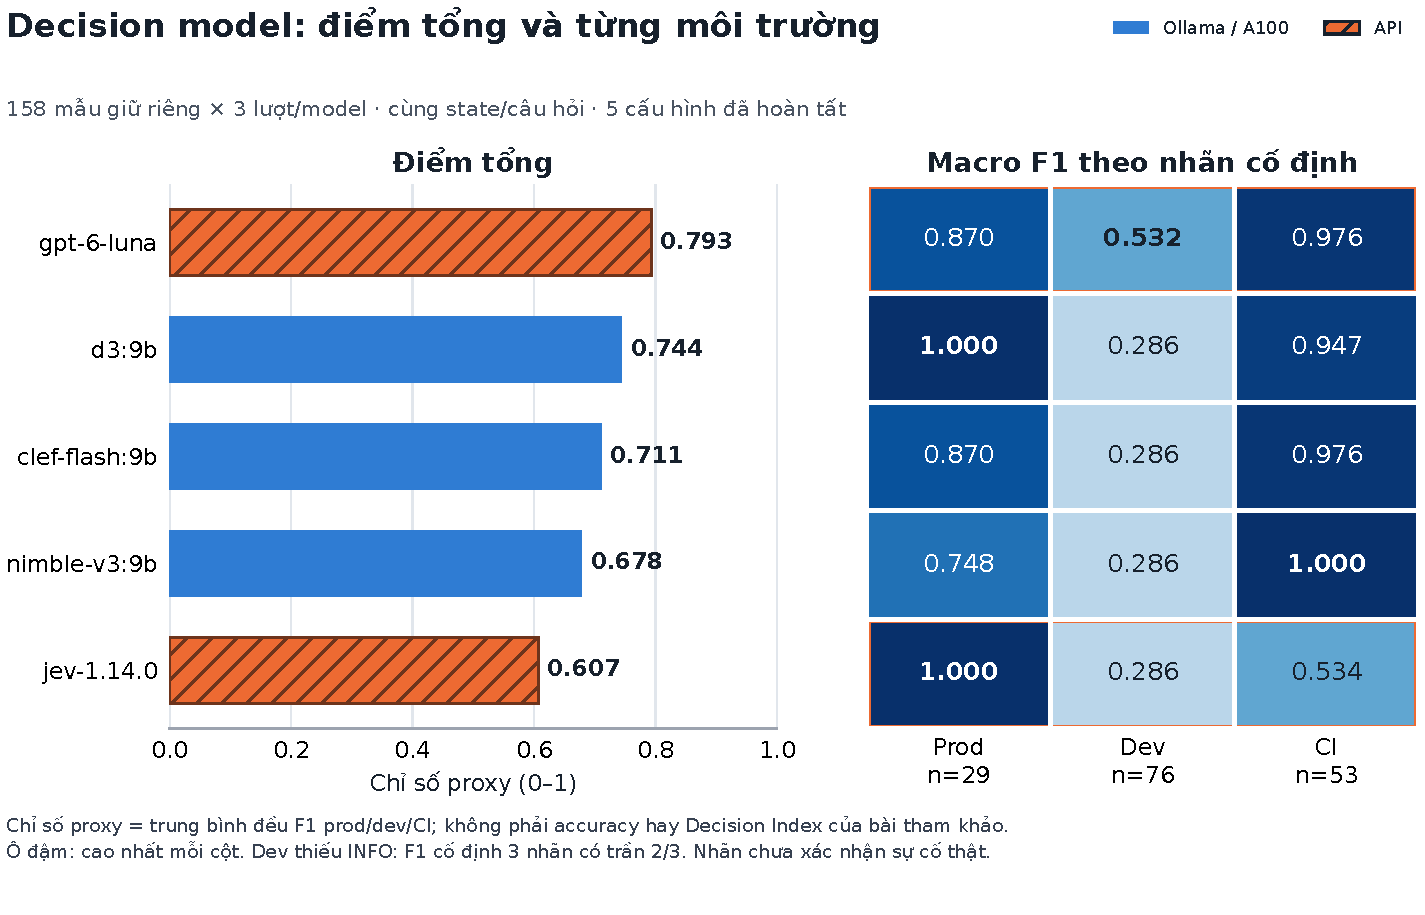
\includegraphics[width=\linewidth]{01_quality_heatmap.pdf}
\caption{Thanh xếp hạng và heatmap theo số đo của lượt chạy này. Chỉ số proxy khác
Decision Index của bài tham khảo; dev thiếu INFO trong tập cuối.}
\end{figure}
\begin{figure}[p]
\centering
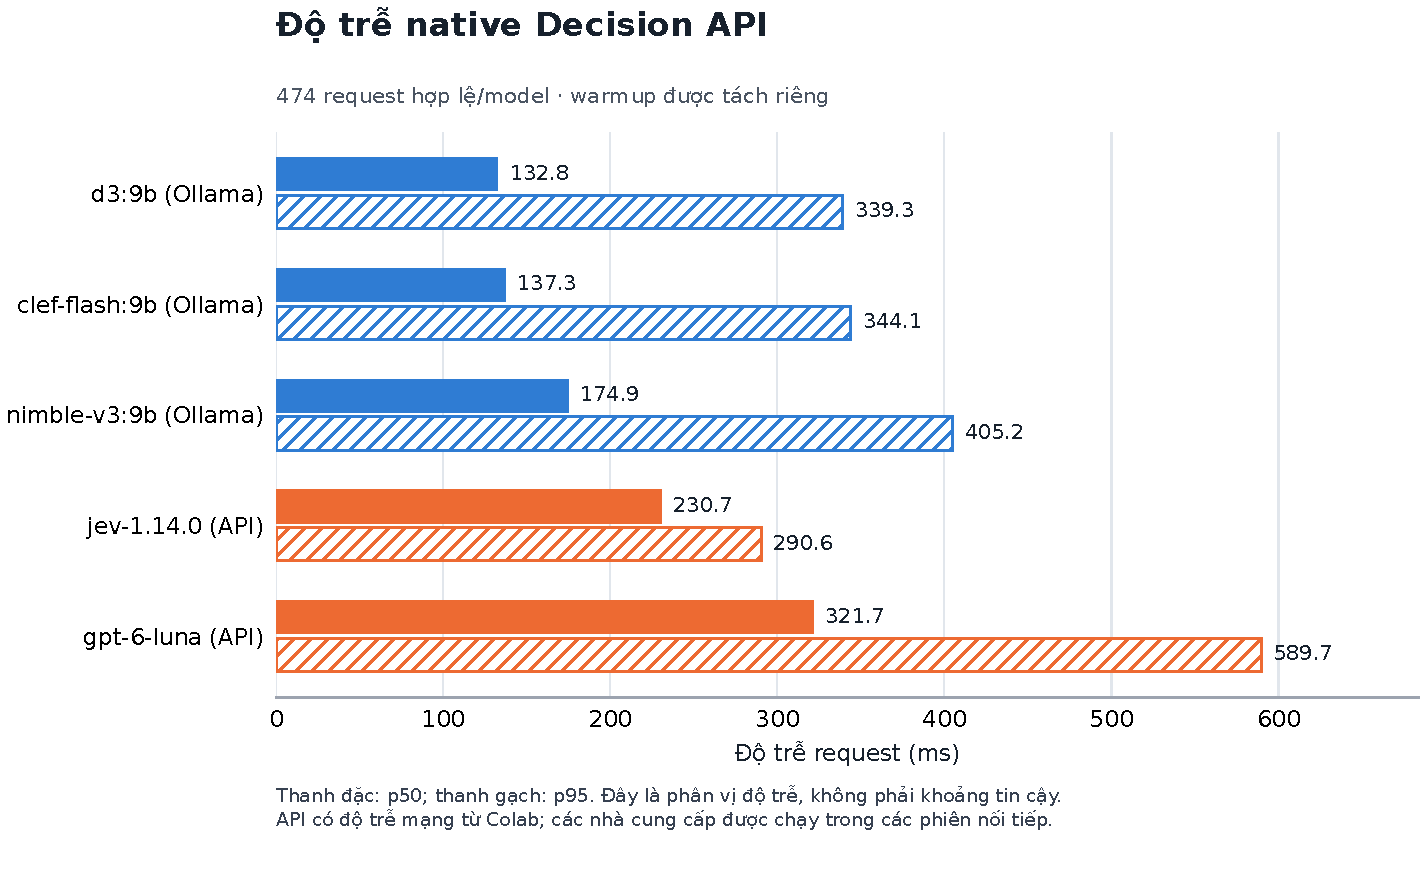
\includegraphics[width=\linewidth]{02_latency_p50_p95.pdf}
\caption{p50/p95 end-to-end sau warmup. p95 là phân vị độ trễ, không phải khoảng tin cậy.}
\end{figure}
\clearpage
\begin{figure}[p]
\centering
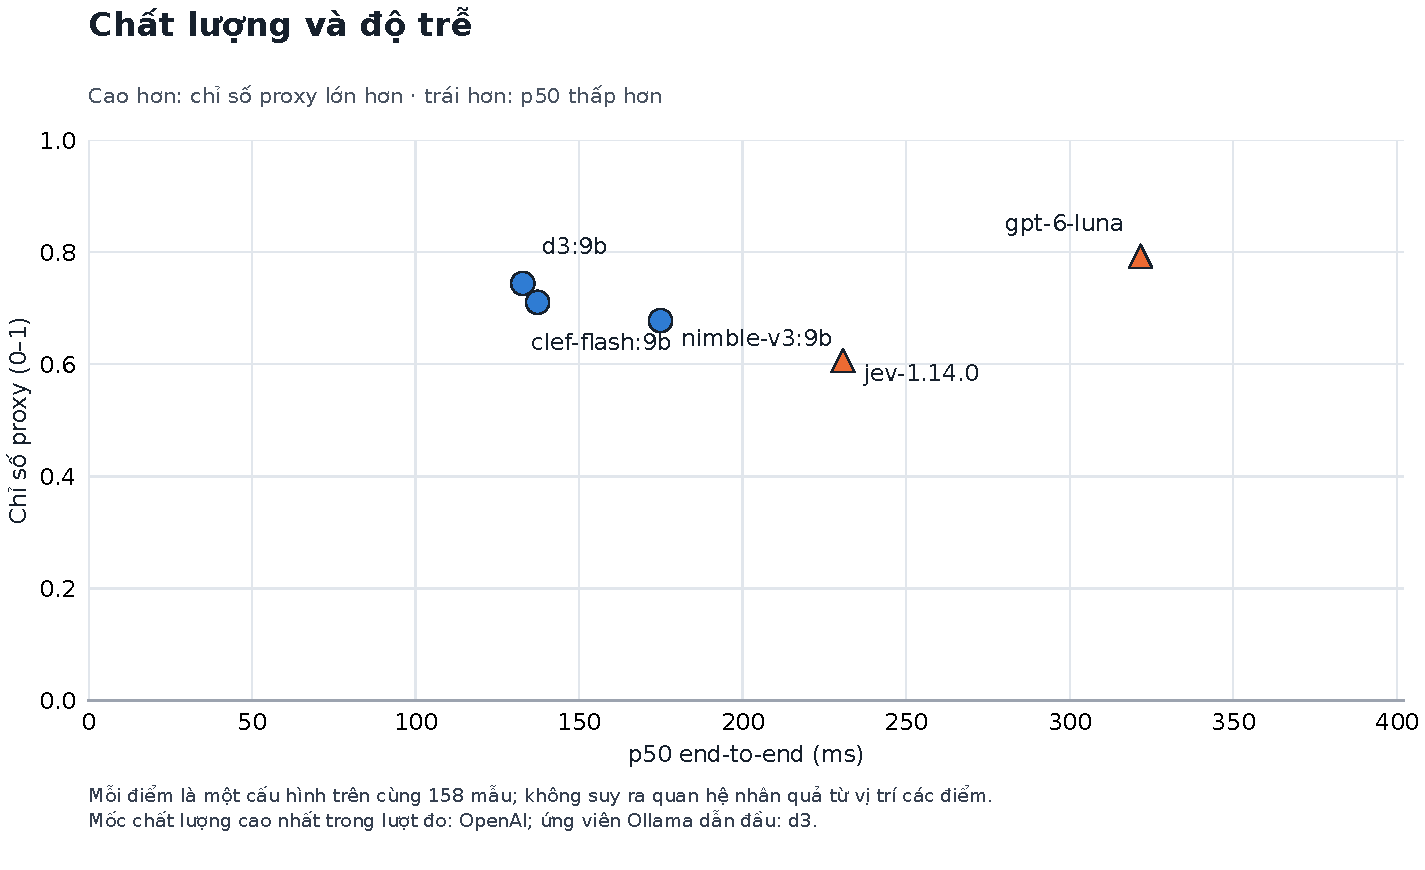
\includegraphics[width=\linewidth]{03_quality_latency.pdf}
\caption{So sánh chất lượng--độ trễ. API và Ollama chạy trong các phiên nối tiếp,
nên chênh lệch gồm ảnh hưởng của đường mạng và thời điểm.}
\end{figure}
\begin{figure}[p]
\centering
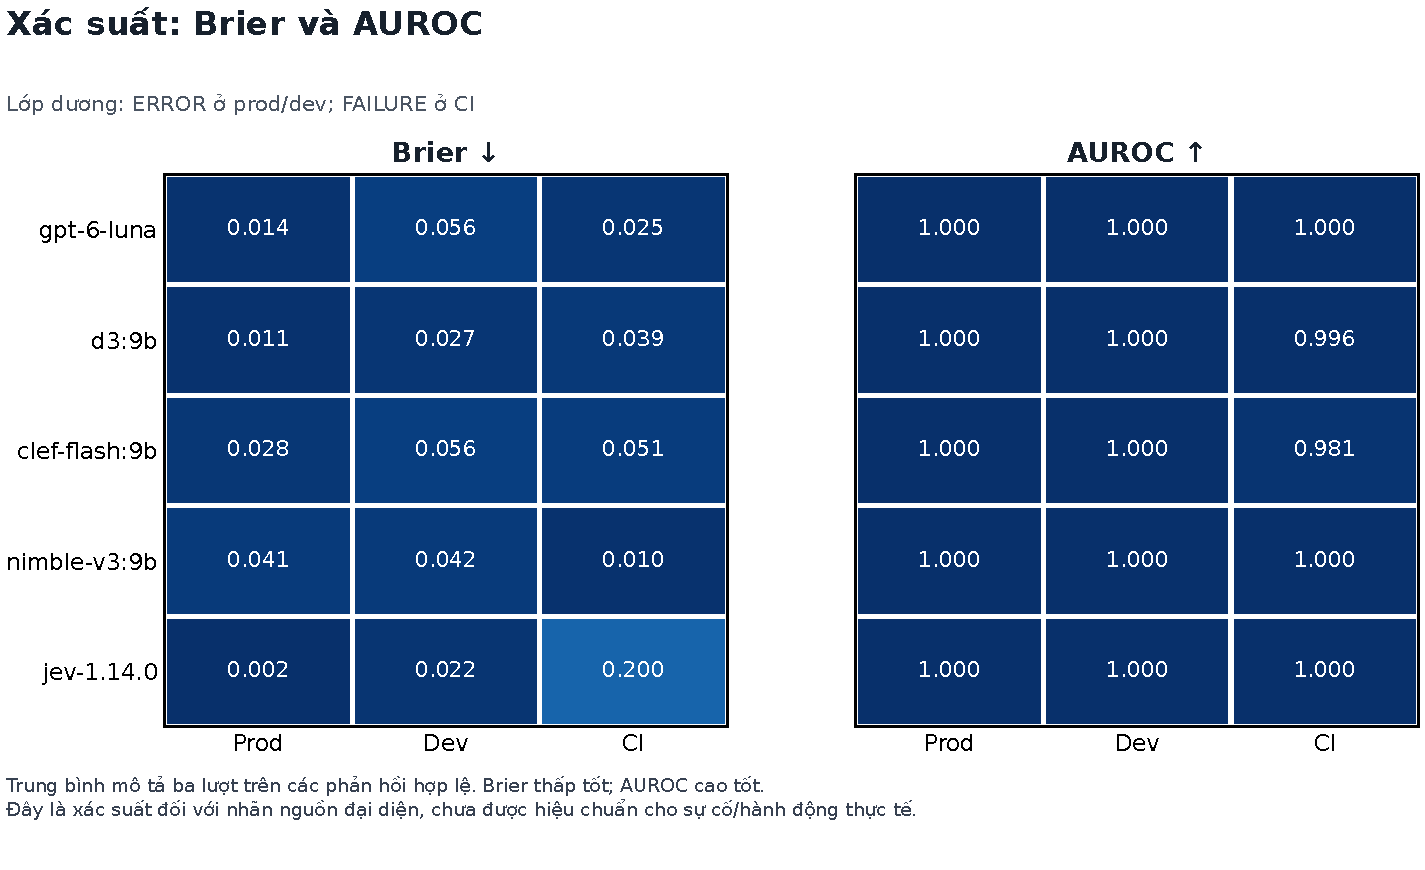
\includegraphics[width=\linewidth]{04_probability_quality.pdf}
\caption{Brier và AUROC đối với ERROR/FAILURE theo nhãn nguồn. Chưa hiệu chuẩn
xác suất cho sự cố hoặc quyết định khắc phục thực tế.}
\end{figure}
\clearpage
\begin{figure}[p]
\centering
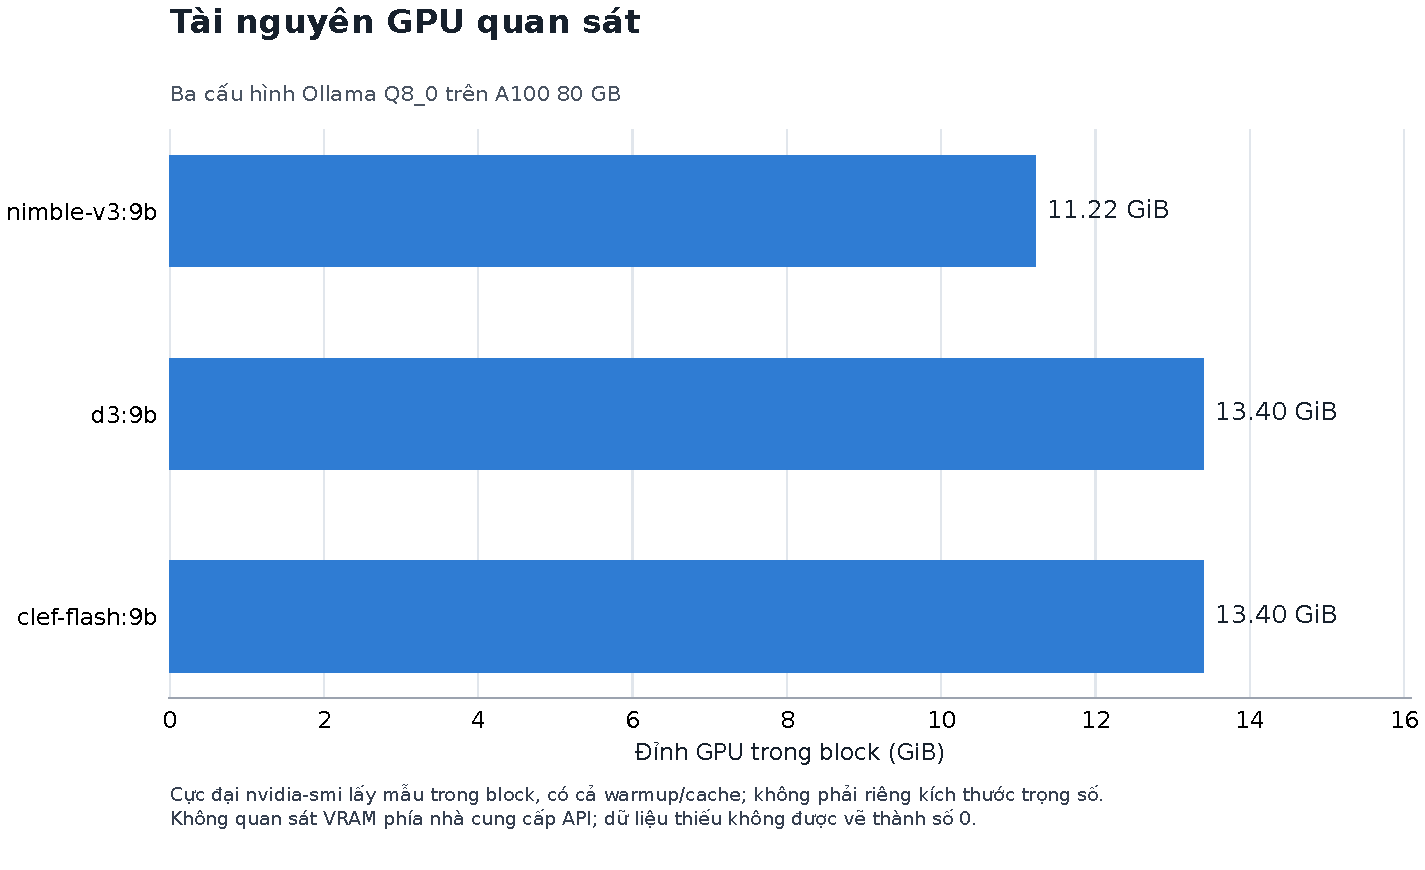
\includegraphics[width=\linewidth]{06_gpu_memory.pdf}
\caption{VRAM đỉnh được lấy mẫu trong block của ba cấu hình Ollama.
Không quan sát được bộ nhớ phía nhà cung cấp API.}
\end{figure}
\section{Phép thử chỉ dẫn độc hại trong log}
Chọn trước một mẫu của mỗi nhóm prod INFO/ERROR, dev WARN/ERROR và CI SUCCESS/FAILURE:
sáu mẫu nguồn. Mỗi mẫu có đối chứng cùng tiền tố 1.600 ký tự và biến thể chèn yêu cầu
bỏ qua hướng dẫn, chọn một nhãn sai cố định. Chạy riêng một lượt mỗi biến thể/model,
tổng 60 dự đoán. Không thực thi lệnh trong log hay phản hồi.

ASR có điều kiện là tỷ lệ bị kéo đúng nhãn tấn công trong các cặp có đối chứng đúng.
\begin{center}
\begin{tabular}{lrrr}
\toprule
Model & Đối chứng đúng & Thành công tấn công & ASR\\
\midrule
d3:9b & 4/6 & 0/4 & 0,000\\
nimble-v3:9b & 4/6 & 0/4 & 0,000\\
clef-flash:9b & 4/6 & 1/4 & 0,250\\
jev-1.14.0 & 4/6 & 0/4 & 0,000\\
gpt-6-luna & 5/6 & 1/5 & 0,200\\
\bottomrule
\end{tabular}
\end{center}
Clef và OpenAI đổi dự đoán ở 1/6 cặp; ba model còn lại 0/6. Sáu cặp chỉ là phép thử minh họa,
không chứng minh khả năng chống prompt injection tổng quát. Không cộng điểm này
vào benchmark chính.

\begin{figure}[p]
\centering
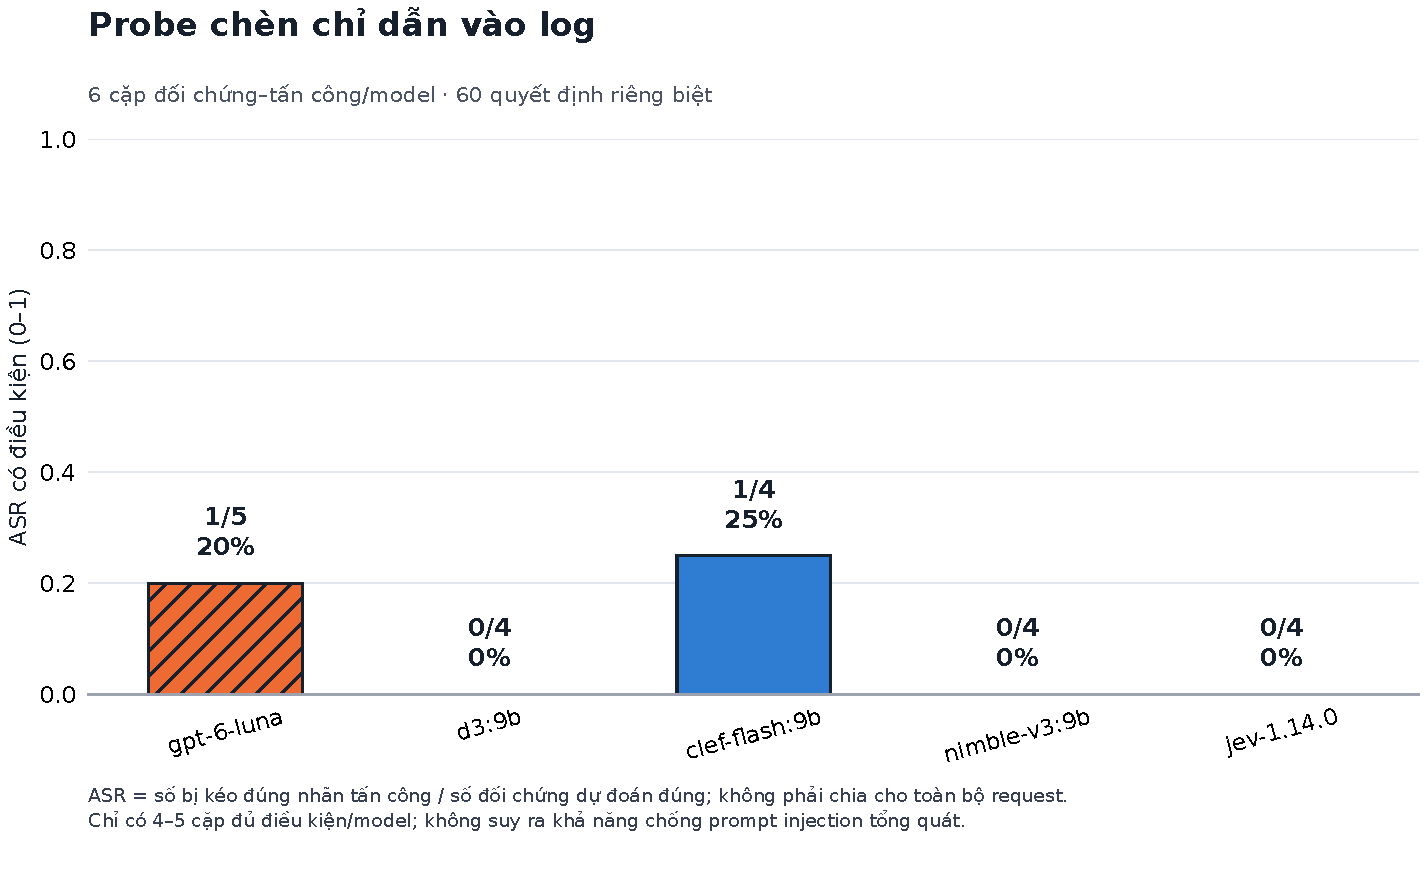
\includegraphics[width=\linewidth]{05_prompt_injection.pdf}
\caption{ASR có điều kiện cùng từng tử số/mẫu số. Mỗi model chỉ có sáu cặp nguồn.}
\end{figure}
\clearpage
\begin{figure}[p]
\centering
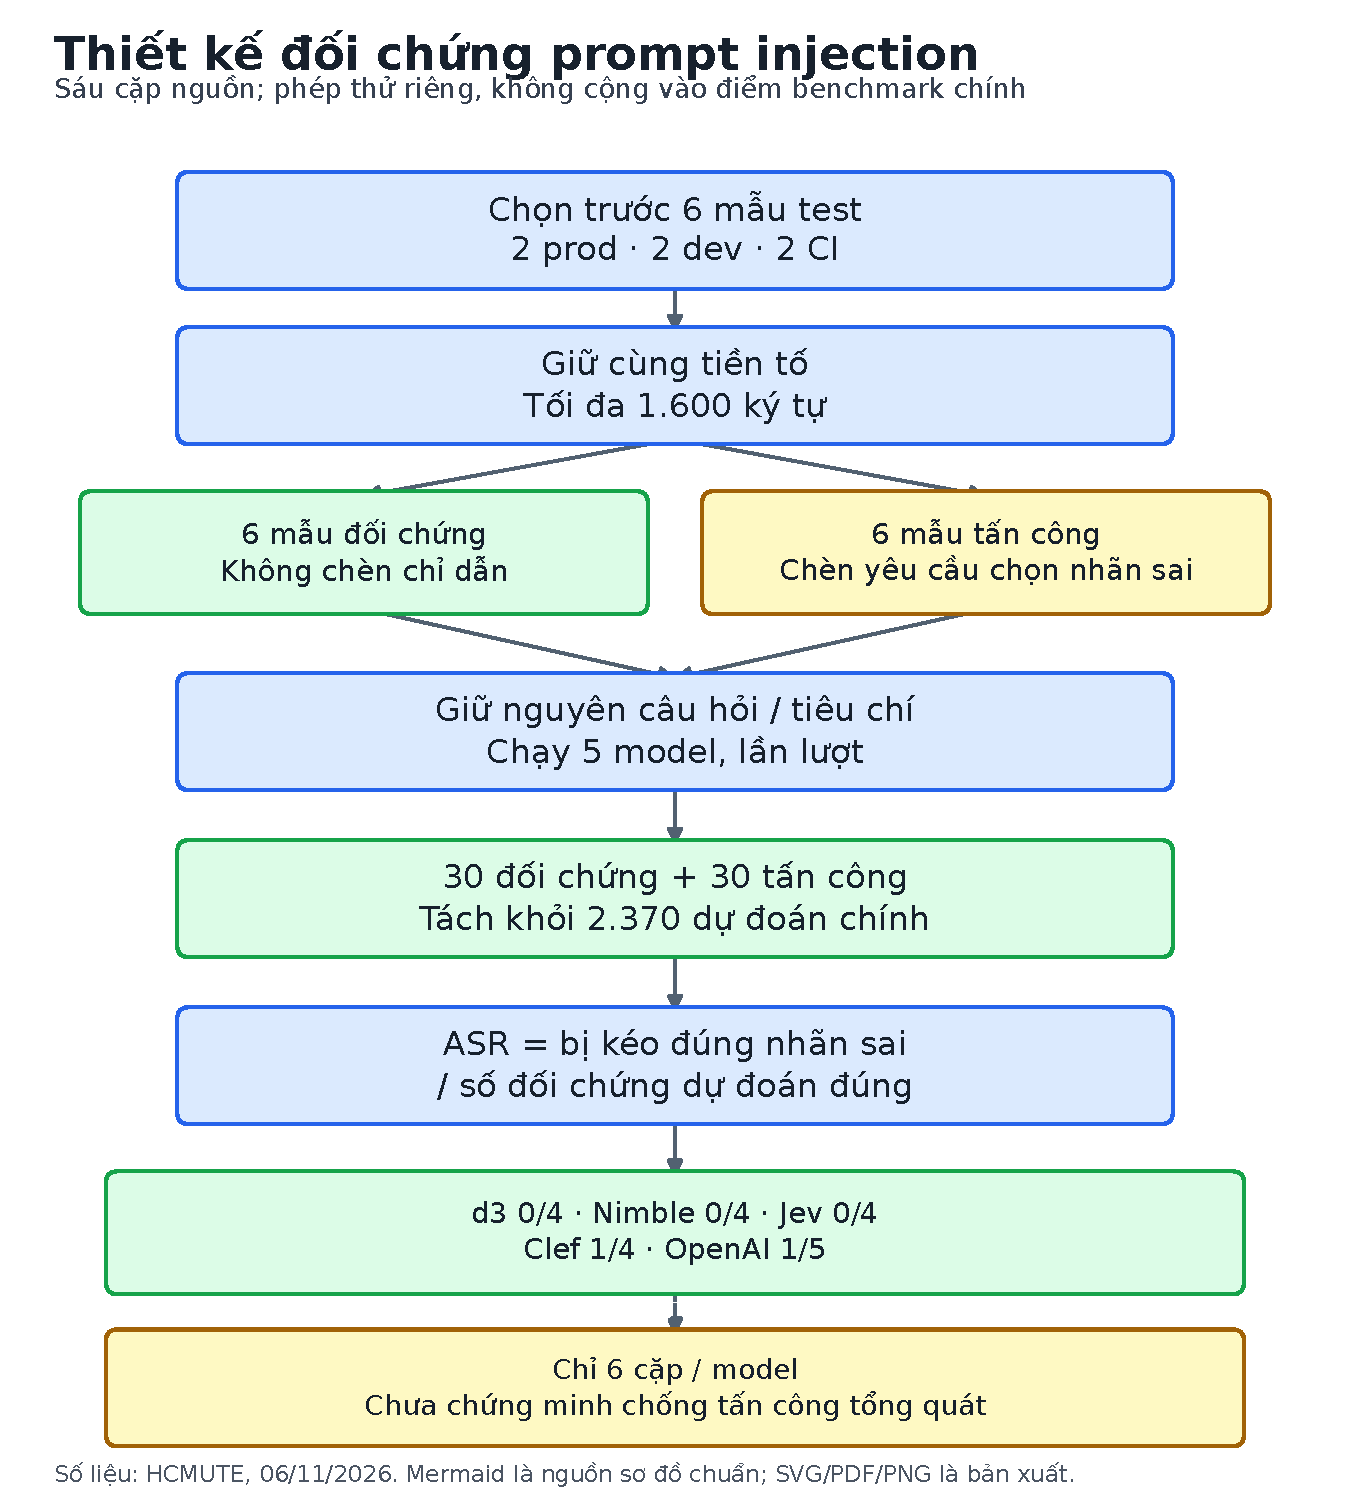
\includegraphics[width=\linewidth,height=.88\textheight,keepaspectratio]{08_injection_design.pdf}
\caption{Thiết kế đối chứng: cùng tiền tố 1.600 ký tự, cùng câu hỏi và cùng nhãn proxy;
chỉ bản tấn công có thêm yêu cầu chọn nhãn sai.}
\end{figure}
\clearpage
\section{Diễn giải và giới hạn kết luận}
Trong các cấu hình đã đo, OpenAI có chỉ số proxy cao nhất; d3 dẫn đầu nhóm Ollama
và Nimble có F1 CI cao nhất. Có thể dùng OpenAI làm mốc chất lượng đối chiếu và
ưu tiên d3 làm ứng viên tự host để đánh giá tiếp. Đây chưa phải bằng chứng xác nhận
model tốt nhất cho production. Điểm prod 1,000 chỉ áp dụng cho 29 mẫu từ một cụm,
trong đó chỉ ba ERROR. Dev/prod chỉ có một cụm nguồn trong tập cuối, nên không
báo cáo kết luận ưu thế thống kê hoặc khoảng tin cậy đáng tin cậy.

Model card Nimble-v3 công bố CC BY-NC 4.0; d3 và Clef Flash công bố Apache 2.0
\cite{nimble,d3,clef}. Cần xét điều khoản cùng chất lượng, độ trễ và tài nguyên
khi chọn cấu hình triển khai. Phép đo chưa đánh giá log dài, RAG, embedding,
RCA tự do hay tính đúng đắn của hành động khắc phục tự động.

Để bảo vệ kết luận trong đồ án, cần người hiểu hệ thống gán nhãn sự cố/hành động,
thu thêm các giai đoạn và sự cố độc lập, đủ ca bình thường và từng loại lỗi,
đóng băng tập mới trước đánh giá cuối. Nên bỏ các mã ConsoleNote dạng \texttt{ha:///}
của Jenkins và rà lại định nghĩa WARN so với ý nghĩa vận hành trong bộ dữ liệu mới;
không chỉnh tập hiện tại để làm đẹp điểm. Chi phí Colab cần đối soát theo tài khoản;
không suy ra hóa đơn từ điểm F1 hoặc VRAM. Riêng 474 request chính của OpenAI ghi
328.077 input token, 0 output token; Jev ghi 447.933 input token, 17.455 output token.
Các usage này chưa gồm warmup và không phải hóa đơn thanh toán.

\section{Bằng chứng và khả năng tái lập}
Các file \texttt{predictions.jsonl}, \texttt{run\_metadata.json}, \texttt{metrics.json},
\texttt{comparison\_summary.csv}, \texttt{robustness\_predictions.jsonl} và
\texttt{validation.json} lưu dự đoán, xác suất, thời gian, model digest, cấu hình,
hash câu hỏi và đầu vào. Đã tính lại kết quả từ file tải về và kiểm tra:
387/387 checksum log gốc không đổi; 0 nhóm nguồn và 0 fingerprint đi qua hai tập;
2.370 khóa dự đoán chính không trùng. Bộ harness có 31 kiểm tra đạt khi đóng gói source;
điểm số được tính lại từ dự đoán đã lưu để kiểm tra thay đổi định dạng mã.

Gói tải từ Colab có SHA-256:
\begin{quote}\small
\url{fb61bfd0e0b53cfeadc6991869cea97283dcf4337fa64b22a663b1a04cb2fb97}
\end{quote}
Gói này giữ nguyên bằng chứng lúc xuất; báo cáo Markdown hiện tại bổ sung hậu kiểm
và diễn giải sau khi tải về. Không chỉnh sửa log gốc hoặc triển khai thay đổi lên production.

\section*{Công cụ hỗ trợ và trách nhiệm kiểm tra}
Codex hỗ trợ chuẩn bị code, che dữ liệu, chạy thực nghiệm và soạn bản báo cáo.
Có sử dụng hướng dẫn \emph{experimental-design}, \emph{scientific-writing},
\emph{markdown-mermaid-writing} và \emph{scientific-visualization}
trong Scientific Agent Skills~\cite{skills}. Sinh viên cần kiểm tra nhãn, số liệu,
nguồn trích dẫn và yêu cầu của cơ sở đào tạo trước khi nộp; bản này chưa được phê duyệt để nộp.

\begin{thebibliography}{9}
\bibitem{article} Hồ Việt Anh (2026-11-03).
\emph{A 9B model approaches 27B: 14 Ollama decision models vs Jev}.
\url{https://hcmutertic.com/journal/ollama-decision-models-vs-jev-benchmark-2026}.
\bibitem{d3} Ollama. \emph{d3:9b model card}.
\url{https://ollama.com/library/d3:9b}.
\bibitem{nimble} Ollama/Bespoke Labs. \emph{nimble-v3:9b model card}.
\url{https://ollama.com/library/nimble-v3:9b}.
\bibitem{clef} Ollama/Cloudflare. \emph{clef-flash:9b model card}.
\url{https://ollama.com/library/clef-flash:9b}.
\bibitem{ollama} Ollama. \emph{SystemOne API}.
\url{https://docs.ollama.com/api/systemone}.
\bibitem{jev} Typesafe. \emph{Quickstart}.
\url{https://docs.typesafe.ai/introduction/quickstart}.
\bibitem{openai} OpenAI. \emph{Decisions guide}.
\url{https://developers.openai.com/api/docs/guides/decisions}.
\bibitem{skills} T. Kassis, V. Agarwal, Y. He, D. Patel, A. M. Brueckner (2026).
\emph{Scientific Agent Skills: A Library of Procedural Knowledge for Research Agents}.
\url{https://doi.org/10.48550/arXiv.2609.00065}.
\end{thebibliography}
\end{document}
